\documentclass[a4paper,11pt]{article}
\input{/home/tof/Documents/Cozy/latex-include/preambule_doc.tex}
\input{/home/tof/Documents/Cozy/latex-include/preambule_commun.tex}
\newcommand{\showprof}{show them}  % comment this line if you don't want to see todo environment
\setlength{\fboxrule}{0.8pt}
\fancyhead[L]{\fbox{\Large{\textbf{Archi 14}}}}
\fancyhead[C]{\textbf{Exercices OSPF}}
\newdate{madate}{10}{09}{2020}
%\fancyhead[R]{\displaydate{madate}} %\today
\fancyhead[R]{Terminale - NSI}
\fancyfoot[L]{\vspace{1mm}Christophe Viroulaud}
\AtEndDocument{\label{lastpage}}
\fancyfoot[C]{\textbf{Page \thepage/\pageref{lastpage}}}
\fancyfoot[R]{\includegraphics[width=2cm,align=t]{/home/tof/Documents/Cozy/latex-include/cc.png}}

\begin{document}

\begin{exo}
Établir un tableau récapitulatif du débit des technologies de connexions existantes. Attention certaines connexions sont asymétriques.
\end{exo}
\begin{exo}
Un réseau est composé des routeurs avec les relations de voisinage suivantes:
\begin{center}
    \begin{tabular}{|c|c|}
        \hline
        \multicolumn{2}{|c|}{A}\\
        \hline
        B & 25Mbit/s\\
        \hline
        E & 20Mbit/s\\
        \hline
    \end{tabular}
    \begin{tabular}{|c|c|}
        \hline
        \multicolumn{2}{|c|}{B}\\
        \hline
        A & 25Mbit/s\\
        \hline
        C & 50Mbit/s\\
        \hline
        F & 16,7Mbit/s\\
        \hline
    \end{tabular} 
    \begin{tabular}{|c|c|}
        \hline
        \multicolumn{2}{|c|}{C}\\
        \hline
        B & 50Mbit/s\\
        \hline
        D & 14,3Mbit/s\\
        \hline
        E & 100Mbit/s\\
        \hline
    \end{tabular} 
\\
    \begin{tabular}{|c|c|}
        \hline
        \multicolumn{2}{|c|}{D}\\
        \hline
        C & 14,3Mbit/s\\
        \hline
        F & 33,3Mbit/s\\
        \hline
    \end{tabular} 
    \begin{tabular}{|c|c|}
        \hline
        \multicolumn{2}{|c|}{E}\\
        \hline
        A & 20Mbit/s\\
        \hline
        C & 100Mbit/s\\
        \hline
        F & 33,3Mbit/s\\
        \hline
    \end{tabular} 
    \begin{tabular}{|c|c|}
        \hline
        \multicolumn{2}{|c|}{F}\\
        \hline
        B & 16,7Mbit/s\\
        \hline
        D & 33,3Mbit/s\\
        \hline
        E & 33,3Mbit/s\\
        \hline
    \end{tabular} 
\end{center}
\begin{enumerate}
    \item Calculer les coûts de chaque liaison.
    \item Construire le graphe \emph{pondéré} correspondant aux états de lien du réseau.
    \item On considère le réseau comme une unique zone \emph{backbone} OSPF. Construire la table de routage de A et de D. Les destinations à atteindre seront les routeurs. Les interfaces ne seront pas précisées.
\end{enumerate}
\end{exo}
\begin{exo}
    \begin{center}
        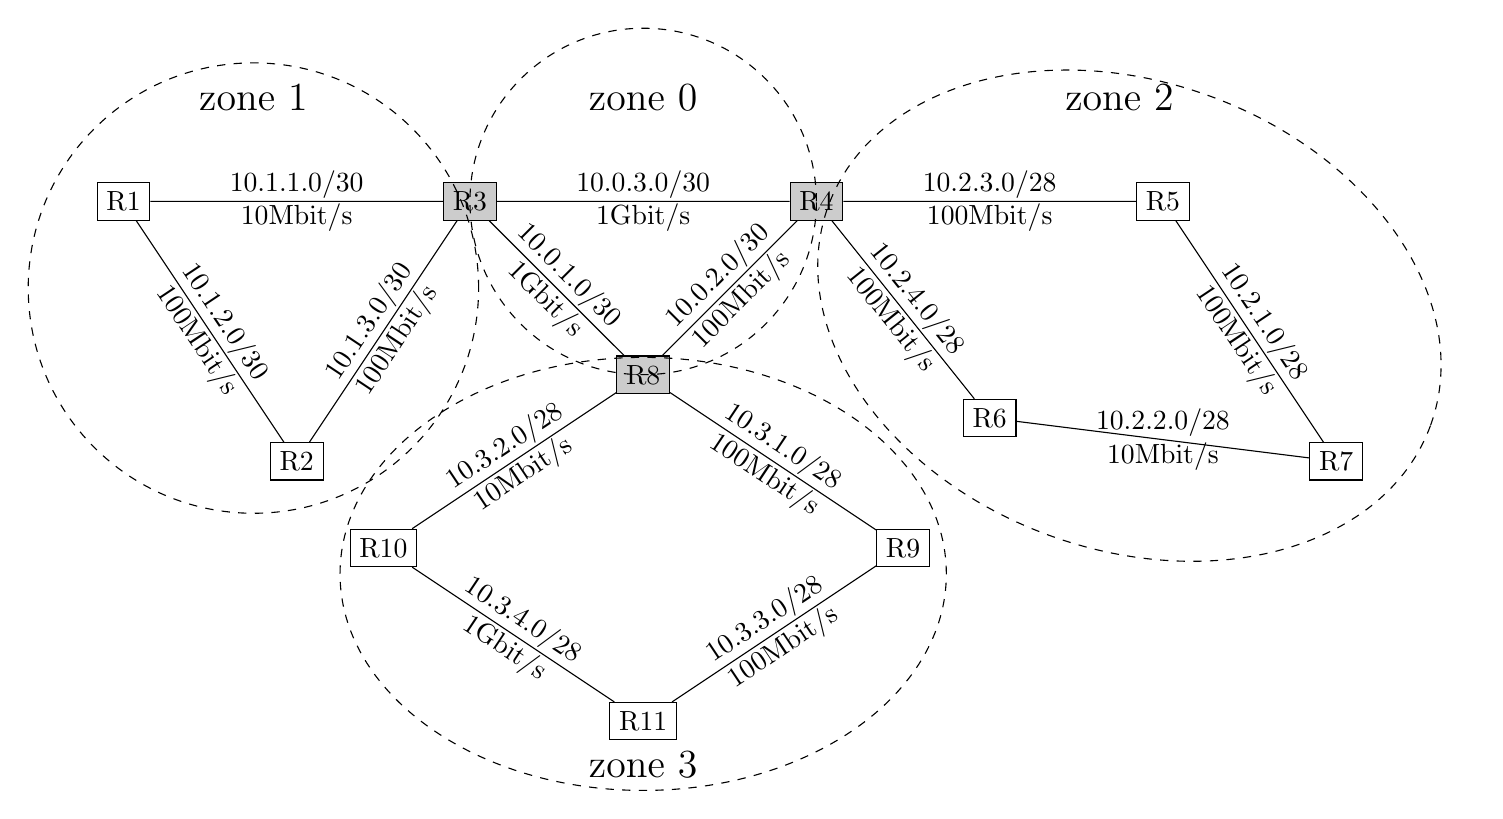
\begin{tikzpicture}[scale=1.1]
            \node[draw] (R1) at (-6,3) {R1};
            \node[draw] (R2) at (-4,0) {R2};
            \node[draw, fill=gray!40] (R3) at (-2,3) {R3};
            \node[draw, fill=gray!40] (R4) at (2,3) {R4};
            \node[draw] (R5) at (6,3) {R5};
            \node[draw] (R6) at (4,0.5) {R6};
            \node[draw] (R7) at (8,0) {R7};
            \node[draw, fill=gray!40] (R8) at (0,1) {R8};
            \node[draw] (R9) at (3,-1) {R9};
            \node[draw] (R10) at (-3,-1) {R10};
            \node[draw] (R11) at (0,-3) {R11};
            \node (Z1) at (-4.5,4.2) {\Large{zone 1}};
            \node (Z0) at (0,4.2) {\Large{zone 0}};
            \node (Z2) at (5.5,4.2) {\Large{zone 2}};
            \node (Z3) at (0,-3.5) {\Large{zone 3}};

            
            \draw (R1) -- (R3) node[midway,text width=1.8cm, text centered]{10.1.1.0/30 10Mbit/s};
            \draw (R1) -- (R2) node[sloped, midway,text width=1.8cm, text centered]{10.1.2.0/30 100Mbit/s};
            \draw (R3) -- (R2) node[sloped, midway,text width=1.8cm, text centered]{10.1.3.0/30 100Mbit/s};
            \draw (R3) -- (R4) node[midway,text width=1.8cm, text centered]{10.0.3.0/30 1Gbit/s};
            \draw (R4) -- (R5) node[midway,text width=1.8cm, text centered]{10.2.3.0/28 100Mbit/s};
            \draw (R4) -- (R6) node[sloped, midway,text width=1.8cm, text centered]{10.2.4.0/28 100Mbit/s};
            \draw (R7) -- (R6) node[midway,text width=1.8cm, text centered]{10.2.2.0/28 10Mbit/s};
            \draw (R5) -- (R7) node[sloped, midway,text width=1.8cm, text centered]{10.2.1.0/28 100Mbit/s};
            \draw (R8) -- (R9) node[sloped,midway,text width=1.8cm, text centered]{10.3.1.0/28 100Mbit/s};
            \draw (R8) -- (R10) node[sloped,midway,text width=1.8cm, text centered]{10.3.2.0/28 10Mbit/s};
            \draw (R9) -- (R11) node[sloped,midway,text width=1.8cm, text centered]{10.3.3.0/28 100Mbit/s};
            \draw (R10) -- (R11) node[sloped,midway,text width=1.8cm, text centered]{10.3.4.0/28 1Gbit/s};
            \draw (R3) -- (R8) node[sloped,midway,text width=1.8cm, text centered]{10.0.1.0/30 1Gbit/s};
            \draw (R4) -- (R8) node[sloped,midway,text width=1.8cm, text centered]{10.0.2.0/30 100Mbit/s};
    
            \draw[dashed] (0,3) circle (2) ;
            \draw[dashed] (-4.5,2) circle (2.6) ;
            \draw[dashed,rotate=-20] (4.7,3.5) ellipse (3.7 and 2.7) ;
            \draw[dashed] (0,-1.3) ellipse (3.5 and 2.5) ;
        \end{tikzpicture}
        \captionof{figure}{Découpage en zones}
        \label{reseau1}
    \end{center}
    On applique le protocole OSPF sur le réseau figure \ref{reseau1}. La zone 0 est \emph{backbone}.
    \begin{enumerate}
        \item Calculer les coûts de chaque connexion.
        \item Établir les tables de routage de R1.
        \item Le réseau 10.0.3.0/30 tombe en panne. Que devient la table de routage de R1?
    \end{enumerate}
\end{exo}
\pagebreak
\begin{exo}
\textbf{Extrait du sujet 0 du bac blanc 2021: }
\begin{center}
\centering
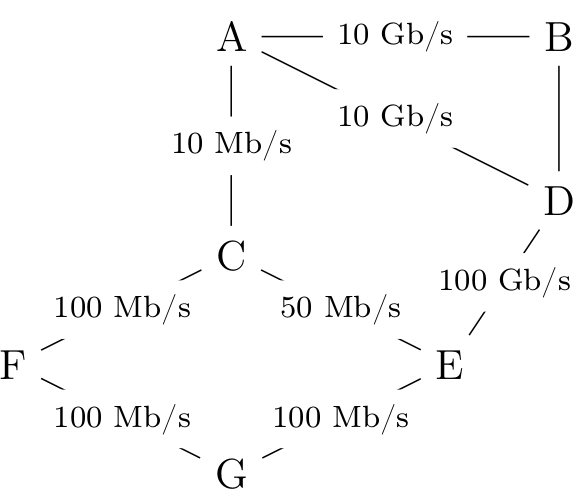
\includegraphics[width=8cm]{ressources/bacblanc.png}
\captionof{figure}{Réseau}
\label{IMG}
\end{center}
\begin{enumerate}
    \item \begin{enumerate}
        \item Vérifier que le coût de la liaison entre les routeurs A et B est 0,01.
        \item La liaison entre le routeur B et D a un coût de 5. Quel est le débit de cette liaison ?
    \end{enumerate}
    \item Le routeur A doit transmettre un message au routeur G, en empruntant le chemin dont la somme des coûts sera la plus petite possible. Déterminer le chemin parcouru.
\end{enumerate}
\end{exo}
\begin{exo}
On considère un réseau ayant les propriétés suivantes:
\begin{itemize}
    \item la distance entre deux nœuds est toujours inférieure à 15,
    \item pour chaque paire de nœuds (A,B) il n'existe pas plusieurs chemins de même taille entre A et B.
\end{itemize}
On considère ce réseau comme une unique zone \emph{backbone} OSPF. Donner une condition suffisante pour que RIP et OSPF calcule les mêmes routes.
\end{exo}
\end{document}